\section{Introduction to Ethereum}
\label{sec:eth-blockchain}
Open source blockchain networks like Ethereum and Bitcoin are software kits that allow you to create an economic system in software, replete with account management and a native unit of exchange that can be used to transfer funds between accounts. These native units of exchange are referred to as coins, tokens, or cryptocurrencies, but they are the same as tokens in any other system: they are a type of money that can only be used within that system to pay peers or run programs on the Ethereum network.
When you want to make one of these peer-to-peer networks accessible through a web browser, you need to use special software libraries such as Web3\footnote{\url{https://github.com/ethereum/web3.py}} which is utilized in this thesis to connect to the Ethereum network \cite[2]{dannen2017introducing}.
The fact that everyone in the world can interact with the same distributed database, given you have internet access and a decent device is favorable for a fixity storage such as presented in Chapter \ref{ch:fixity-storage}, since anyone will be able to confirm if an object has changed over time if given the right resources, such as the transaction hash in which the fixity information of an object was stored on the blockchain. Let us picture a digital archive which releases multiple objects to the public and their respective fixity information on the blockchain, the community could then validate if the object in question is authentic. Pure trust, that an archive or its stewards did not tamper with the data in their care is therefore not needed anymore.
\section{About the blockchain}
A block is a time unit that contains a specific amount of transactions. Transaction data is captured throughout that time period, and when the unit of time expires, the next block begins. The blockchain is a representation of the history of state changes in the EVM's network database \cite[43]{dannen2017introducing}.
The Ethereum network divides transactions and state changes into blocks, which are then hashed. Before the following canonical block may be added on top of it, each block is inspected and validated. Nodes on the network will no longer need to evaluate the trustworthiness of every single block in the Ethereum network's history; instead, they will only need to compute the current balances of the accounts on the network. They only check to see if its "parent block" is the most recent canonical block. They do it rapidly by checking to verify if the new block has the right hash of its parents' transactions and state.
The blockchain is made up of all the blocks strung together, including the genesis block, which is an honorific designating the first block mined by the network after it went live. The blockchain is also known as a distributed ledger or distributed ledger technology in some sectors (DLT). The term "ledger" is correct since the chain contains every transaction in the network's history, thereby turning it into a massive, well-balanced ledger \cite[55]{dannen2017introducing}. 
\section{Ethereum Virtual Machine}
\label{sec:evm}
The physical manifestation of the EVM cannot be compared to that of a cloud or an ocean wave, but it does exist as a single entity sustained by thousands of connected computers running an Ethereum client\footnote{\url{https://ethereum.org/en/developers/docs/evm/}}.
In the Ethereum context, a virtual machine (VM) is a massive global computer made up of constituent nodes, which are themselves computers. In general, a virtual machine is a computer system that is emulated by another computer system. These emulations are based on the same computer architectures as the target of their emulation, but they usually reproduce that architecture on hardware other than that for which it was designed. Virtual machines can be built using hardware, software, or a combination of the two. It is both in the case of Ethereum. Rather than securing thousands of individual machines, Ethereum takes the approach of securing one massive state machine that can span the entire globe \cite[48]{dannen2017introducing}.
The EVM can run any computer program written in Solidity\footnote{\url{https://github.com/ethereum/solidity}}, the native programming language of the EVM. These programs will always create the same output, with the same underlying state changes, when given a specific input. As a result, Solidity programs are entirely deterministic and guaranteed to execute, as long as you pay enough for the transaction. Solidity programs are Turing complete in the sense that they can express all tasks that can be performed by computers. This means that every application executed on the platform is run by the entire dispersed network, every node \cite[50]{dannen2017introducing}. 
The EVM is also a runtime environment for small programs that can be executed via a network, from the perspective of a software developer. Smart contracts are compiled into the EVM's native language, the EVM bytecode. By using a client application like Truffle\footnote{\url{https://trufflesuite.com/}} or Geth\footnote{\url{https://geth.ethereum.org/}}, Solidity, a high-level language, is compiled into bytecode and posted onto the Ethereum network \cite[51]{dannen2017introducing}. I have decided to utilize Truffle for this thesis because of its fast and easy way to interact with the Ethereum network and its subnetworks.
\section{Smart Contracts}
Smart contracts, similar to the concept of classes in traditional object-oriented programming, are the building blocks of decentralized apps operating on the EVM. When developers talk about developing smart contracts, they're usually talking to writing code in the Solidity programming language for execution on the Ethereum network. Units of value can be exchanged as readily as data when the code is run \cite[10]{dannen2017introducing}.
In my thesis, the fixity storage is often referred to as decentralized application (DAPP) which is built with several smart contracts. The smart contract implement in this thesis is further described in Section \ref{sec:implementation}. 

\section{Persistence}\label{sec:persistence}
Decentralized storage systems, unlike centralized servers managed by a single corporation or organization, are made up of a peer-to-peer network of users that each hold a share of the overall data, resulting in a resilient file storage sharing system. These can be found in any peer-to-peer network or in a blockchain-based application. Ethereum is a decentralized storage system in and of itself, and it is when it comes to code storage in all smart contracts. When it comes to massive amounts of data, however, Ethereum was not intended for that. 
The chain is steadily growing and on March 19, 2022, the Ethereum chain is at 602.95 GB\footnote{\url{https://ycharts.com/indicators/ethereum_chain_full_sync_data_size}}, which every node on the network needs to be able to store. If the chain were to expand to large amounts of data (say 5TBs) it wouldn't be feasible for all nodes to continue to run. Also, the cost of deploying this much data to Mainnet would be prohibitively expensive due to gas fees\footnote{\url{https://ethereum.org/en/developers/docs/storage/}}.
My proposed solution utilizing is pooled testing in order to mitigate the ever-increasing chain size of the Ethereum network by reducing the amount of transactions needed to operate the fixity storage. 
All transactions in Ethereum are stored on the blockchain, a canonical history of state changes stored on every single Ethereum node \cite[12]{dannen2017introducing}.
A blockchain has a schema, much like any other database: rules establish, constrain, and enforce relationships between entities. Motives to break or alter these relationships can be found in a wide range of industries, leading to bribery and corruption and making blockchain's trustless properties even more appealing to businesses than previous generations of software and networking. Shared read/write access generates considerable complexity in all databases. Depending on where the database is physically situated, machines all over the world may experience variable latency, resulting in certain write operations arriving out of order. This becomes even more challenging when numerous parties are expected to share a database equally \cite[20]{dannen2017introducing}. 
The nodes process the block in question and execute any code included within the transactions. This is done independently by each node; it is not only highly parallelized, but also very redundant. Despite the significant redundancy, this is a reliable and efficient technique to balance a worldwide ledger \cite[50]{dannen2017introducing}.
\subsection{Blockchain-based persistence}
This type of persistence is utilized in my thesis, since the fixity information of the archived objects are meant to be persisted for long term.
Ethereum requires a persistence mechanism in order for a piece of data to last indefinitely. When executing a node, for example, the persistence method requires that the entire chain be considered. The chain continues to grow as new pieces of data are added to the end, requiring each node to reproduce all the embedded data. The term for this is "blockchain-based persistence." The problem with blockchain-based persistence is that the chain could grow to be far too large to maintain and retain all the data in a reasonable amount of time (e.g. many sources estimate the Internet to require over 40 Zetabytes of storage capacity). In addition, the blockchain must have some sort of incentive system.
For blockchain-based persistence, the incentive system includes a payment made to the miner, where they are paid to include data into the next block of the chain\footnote{\url{https://ethereum.org/en/developers/docs/storage/}}.
\subsection{Contract-based persistence}
Data used in smart contracts cannot be duplicated by every node and preserved indefinitely, hence contract-based persistence assumes that data must be kept using contract agreements. These are agreements reached between numerous nodes to hold a piece of data for a set amount of time. They must be refunded or renewed after they expire in order for the data to be preserved. Instead of storing all data on-chain, the hash of where the data is situated on the chain is often stored. This eliminates the requirement for the entire chain to scale in order to keep all the data\footnote{\url{https://ethereum.org/en/developers/docs/storage/}}.
\section{Test Networks}
These networks are not really free of charge, but the ETH token on the respective network is free to get. Although the queue of the free ETH token can be very vast in some cases, e.g. \url{https://faucet.dimensions.network/} this faucet has a waiting queue for over three days until you receive one ETH token for the Ropsten network. Other faucets, a distributor of free ETH test tokens, require social network accounts to verify that you are not a bot e.g. \url{https://faucet.paradigm.xyz/} requires a Twitter account with at least one tweet and at least 15 retweets before you can request one ETH token. The faucet request are almost all time gated, meaning that you could request ETH only once per day. At small scale, this limitation is no problem for this thesis because persisting around 10 pools on the blockchains require at max 0.002 ETH tokens. The one per day paradigm gets problematic for the experiment for the 10,000 objects, which costs about 20 ETH tokens, which means I would have to request tokens for 20 days straight to perform one experiment on a real live environment such as the Ropsten testnet. 
There are multiple options to choose from for a testnet, from the most prominent networks presented at the official Ethereum documentation \footnote{\url{https://ethereum.org/en/developers/docs/networks/}} only the Ropsten network implements the proof-of-work algorithm, which means it is the best representation of Ethereum to date, and for that reason I decided to utilize the Ropsten network in my thesis.
\section{Gas and Fees}
\label{sec:costs}
Gas refers to the unit that measures the amount of computational effort required to execute specific operations on the Ethereum network, this property allows me to calculate the operation cost for the fixity storage without taking the price fluctuation of ETH into account. Since each Ethereum transaction requires computational resources to execute, each transaction requires a fee.
Gas fees are paid in Ethereum's native currency, ETH (ETH). Gas prices are denoted in gwei, which itself is a denomination of ETH - each gwei is equal to 0.000000001 ETH. For example, instead of saying that your gas costs 0.000000001 ether, you can say your gas costs 1 gwei. The word 'gwei' itself means 'giga-wei', and it is equal to 1,000,000,000 wei. Wei itself is the smallest unit of ETH\footnote{\url{https://ethereum.org/en/developers/docs/gas/}}.
Miners are paid in ETH for mining, and also for running scripts on the network. The cost associated with electricity expenditure of servers running on the Ethereum network is one of the factors that gives ETH, as a cryptocommodity, its intrinsic value—that is, someone paid real money to their electricity company to run their mining machine. Specialized mining rigs, which use arrays of graphics cards to increase their odds of completing a block and getting paid \cite[12]{dannen2017introducing}. 
Mining creates the consensus needed to make legitimate state changes, and miners are compensated for their contributions. This is how Ethereum (ETH) and Bitcoin (BTC) are created \cite[57]{dannen2017introducing}. 
To ensure that the system is not clogged by meaningless spam contracts, there must be a fee associated with each instruction the EVM executes. An internal counter maintains account of the fees incurred each time an instruction is executed, which are then charged to the user. When a user initiates a \gls{transaction}, a tiny percentage of the user's wallet is set aside to pay these fees \cite[58]{dannen2017introducing}. The costs are the driving factor of my thesis where I try to make as fewer transactions as possible to run a fixity storage on the Ethereum network. 
The fees are determined by the transaction's gas cost; gas is a unit of effort, not a subcurrency, therefore it cannot be held or hoarded. In computer words, it simply assesses how much work each step of a transaction will take. You only need to add \acrshort{eth} to your account to be able to pay for gas. There is no need to buy it individually because there is no gas token. Every operation on the EVM has a gas cost attached with it. Gas prices ensure that network computing time is adequately priced \cite[59]{dannen2017introducing}.
The only person who suffers if you transmit a set of computationally difficult commands to the EVM is you. When the amount of ETH you allocated to the transaction runs out, the work will halt. It has no bearing on the transactions of others. There is no method to jam the EVM without spending a significant amount of money in transaction fees. The gas price system serves as a de facto means of scalability. Miners have complete control over which transactions pay the highest fee rates, as well as the block gas limit. The gas limit sets the maximum amount of processing and storage that can be done per block \cite[60]{dannen2017introducing}. 
\section{Transactions}\label{sec:tx-cost}
An Ethereum transaction refers to an action initiated by an externally-owned account, in other words an account managed by a human, not a contract. For example, if Bob sends Alice 1 ETH, Bob's account must be debited and Alice's must be credited. This state-changing action takes place within a transaction. 
Transactions come from external accounts, which are usually controlled by human users. It's a mechanism for an external account to provide the EVM instructions to do a task. To put it another way, it's a method for an external account to send a message to the system. A transaction in the EVM is a cryptographically signed data package storing a message, which tells the EVM to transfer ether, create a new contract, trigger an existing one, or perform some calculation. Contract addresses, like users with external accounts, can be transaction recipients \cite[60]{dannen2017introducing}. 
\begin{figure}[h]
    \caption{Illustration of an Ethereum transaction \url{https://ethereum.org/en/developers/docs/transactions/}}
    \centering
    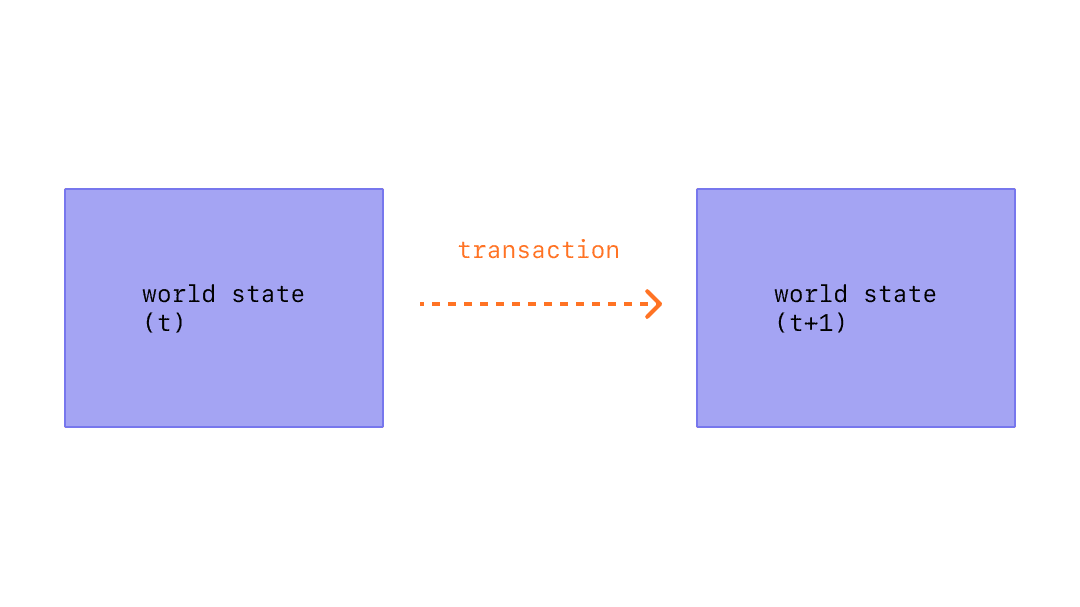
\includegraphics[width=0.5\textwidth]{eth_transaction.png}
\end{figure}
Transactions that affect the EVM's state must be broadcast to the entire network. A miner will execute the transaction and propagate the resulting state change to the rest of the network once any node broadcasts a request for a transaction to be conducted on the EVM\footnote{\url{https://ethereum.org/en/developers/docs/transactions/}}.
Transactions, which do not alter the global state are free of charged and are referred to as Calls. In the source code, as seen in the source code in \ref{lst:fixity-storage}, \textit{getPoolHash(uint32 poolId)} is marked with the keyword view, which means the function itself does not alter the state of the network. Contrary to the function \textit{setPoolHash(uin32 poolId, bytes32 poolHash)} which does alter the networks state and therefore generates cost for the fixity storage. In this thesis, writing actions on the blockchain are often referred to as transactions; and reading actions are referred to as calls.
Table \ref{table:gas-costs} presents the gas cost of the most relevant network operations used in this thesis according to the Ethereum yellow paper \cite[27]{wood2014ethereum}.
\begin{center}
    \begin{tabular}{ l l l }\label{table:gas-costs}
        Operation Name & Gas Cost & Description \\ 
        $codedeposit$ & 200 & gas cost per byte the compiled smart contract \\  
        $txcreate$ & 32000 & create a new smart contract  \\   
        $transaction$ & 21000 & retrieve the current balance of an account \\
        $txdatazero$ & 4 & gas cost for every zero byte of the transaction data  \\   
        $txdatanonzero$ & 16 & gas cost for every non-zero byte of the transaction data  \\   
        $sset$ & 20000 & set a persistent variable for the first time in the contract \\
        $sreset$ & 2900 & the cost for updating a persistent variable 
    \end{tabular}
\end{center}


\section{Wrap Up}
The learnings in this Chapter is on how to interact with the Ethereum network, which tools to use and how the computational cost comes about. I have presented that it is important to prune all unnecessary transaction and storage data to mitigate the ever-increasing chain size of the Ethereum blockchain and reduce the cost for the operator of the fixity storage presented in Chapter \ref{ch:fixity-storage}. 